% Benchmarking Burn, TFLite, and ONNX Runtime Inference on ARM64 Edge Devices
% ComTech: Computer, Mathematics and Engineering Applications
% IEEEtran two-column

\documentclass[conference]{IEEEtran}
\usepackage{cite}
\usepackage{amsmath,amssymb,amsfonts}
\usepackage{algorithmic}
\usepackage{textcomp}
\usepackage{graphicx}
\usepackage{booktabs}
\usepackage{tabularx}
\usepackage{hyperref}
\usepackage{array}

\hypersetup{
    colorlinks=true,
    linkcolor=black,
    urlcolor=blue,
    citecolor=black
}

\graphicspath{{../figures/}}

\begin{document}

\title{Benchmarking Burn, TFLite, and ONNX Runtime Inference on ARM64 Edge Devices}

\author{\IEEEauthorblockN{Fatih Jawwad Al Mumtaz$^{1}$, Amirul Al Aziz$^{2}$}
\IEEEauthorblockA{$^{1}$Informatics Engineering Department\\
University of Darussalam Gontor\\
Ponorogo, Indonesia\\
\texttt{fatihalmumtaz76@student.cs.unida.gontor.ac.id}}
\IEEEauthorblockA{$^{2}$Agricultural Industrial Technology Department\\
University of Darussalam Gontor\\
Ponorogo, Indonesia\\
\texttt{amirulalaziz57@student.tip.unida.gontor.ac.id}}
}

\maketitle

\begin{abstract}
Edge inference on ARM-based single-board computers is critical for deploying deep learning in resource-constrained environments. This paper presents a comparative steady-state warm-cache latency benchmark of three inference frameworks---Burn (native ndarray), TensorFlow Lite (TFLite), and ONNX Runtime (ORT)---on a Raspberry Pi 5 (Cortex-A76) using MobileNetV2. We evaluate single-threaded and multi-threaded latency, throughput, memory usage, CPU utilization, and thermal characteristics under a controlled protocol with IQR-based outlier removal and 95\% bootstrapped confidence intervals. Results show TFLite achieves the lowest latency (22.2 ms single-threaded, 10.7 ms with 4 threads), while Burn demonstrates exceptional memory efficiency at 24.5 MB peak RSS---22$\times$ less than TFLite and 4$\times$ less than ORT---with multi-thread scaling reaching 300 ms (2.6$\times$ speedup). ONNX Runtime offers a balanced trade-off at 45.4 ms single-threaded latency and 100 MB memory footprint. The findings establish Burn as a Rust-native inference framework for ARM64 edge deployment where memory constraints are paramount, and provide reproducible baselines for framework selection.
\end{abstract}

\begin{IEEEkeywords}
Edge inference, ARM64, Raspberry Pi, Burn, burn-onnx, TensorFlow Lite, ONNX Runtime, MobileNetV2, benchmark
\end{IEEEkeywords}

%----------------------------------------------------------------------
\section{Introduction}
\label{sec:intro}
%----------------------------------------------------------------------

The proliferation of deep learning on edge devices has created a growing demand for efficient inference runtimes that balance latency, memory, and power consumption~\cite{howard2017mobilenets, sandler2018mobilenetv2}. Single-board computers such as the Raspberry Pi series have become popular platforms for edge AI prototyping due to their affordability and accessibility. However, selecting an appropriate inference framework for these resource-constrained platforms requires rigorous comparative benchmarking under controlled conditions.

Prior work includes Ignatov et al.~\cite{ignatov2019ai}, who benchmarked mobile AI accelerators across multiple frameworks, and AskariHemmat et al.~\cite{askarihemmat2020systematic}, who evaluated TFLite and ONNX Runtime on edge devices. Almeida et al.~\cite{almeida2023benchmarking} compared inference engines for embedded deployment, while Ahn et al.~\cite{ahn2023quantization} characterized quantization effects across frameworks including TFLite and ONNX on Raspberry Pi using the MLPerf methodology. TFLite~\cite{tflite2017} and ONNX Runtime~\cite{onnx2019} are the dominant general-purpose inference frameworks for ARM edge deployment, with extensive ecosystem support. On the hardware front, Boddu et al.~\cite{yolov4pi2025} demonstrated real-time object detection on the Pi 5 using TFLite INT8 quantization.

More recently, the Burn framework~\cite{burn2024} introduced Rust-native deep learning with ONNX import capabilities. Burn 0.21 uses a build-time codegen approach (\texttt{burn-onnx}) that translates ONNX models into native Rust type-safe inference code at compile time, eliminating runtime ONNX parsers. Rust-based inference~\cite{carnelos2024microflow} offers potential advantages in memory safety and predictable performance without garbage collection. However, Burn's inference performance on ARM64 hardware has not been systematically benchmarked against established frameworks, motivating this study.

Three methodological considerations distinguish this work from prior benchmarks. First, we explicitly measure steady-state warm-cache latency after a 1000-iteration warmup---single-tensor repetition eliminates input-variance confounding, but we frame results accordingly as cache-warm steady-state performance rather than general-purpose throughput. Second, we simultaneously collect latency, memory, CPU utilization, and temperature under a single controlled protocol. Third, we provide a fully reproducible pipeline with code, data, and figures publicly available.

%----------------------------------------------------------------------
\section{Methods}
\label{sec:methods}
%----------------------------------------------------------------------

Experiments were conducted on a Raspberry Pi 5 (Broadcom BCM2712, quad-core ARM Cortex-A76 at 2.4 GHz, 8 GB LPDDR4X, 64 GB microSD storage) running Debian GNU/Linux with kernel 6.18.34+rpt-rpi-2712. The Pi 5 was cooled passively with a heatsink and no active fan, matching typical low-cost edge deployment configurations.

Burn~\cite{burn2024} is a Rust-native deep learning framework. We used Burn 0.21 with the \texttt{ndarray} backend, which provides CPU-based tensor operations via the \texttt{ndarray} Rust crate. The \texttt{mobilenetv2-7.onnx} model was imported into Rust at build time via \texttt{burn-onnx} codegen (\texttt{ModelGen}), which translates the ONNX computation graph into a compile-time type-safe Rust struct with explicit forward-pass code. This eliminates runtime ONNX parsing overhead and enables compiler optimizations across the entire inference pipeline. Thread count is controlled via the \texttt{OMP\_NUM\_THREADS} environment variable, set from the CLI \texttt{--threads} argument. Inference precision is f32 throughout. TFLite was used via the Python \texttt{tensorflow} package (v2.x) with the XNNPACK delegate, with interpreter thread count controlled via \texttt{setNumThreads()}. ONNX Runtime was used via \texttt{onnxruntime} with the CPU execution provider and thread count set via \texttt{SessionOptions.intra\_op\_num\_threads}.

All frameworks ran MobileNetV2~\cite{sandler2018mobilenetv2} at $224\times224\times3$ input resolution. A single synthetic input tensor was generated per run using a deterministic seed (42) and held constant across all 2000 iterations. This methodology measures steady-state warm-cache inference latency---the best-case scenario for a deployed pipeline---rather than heterogeneous-input throughput. We verified that all three frameworks produce valid finite outputs on the same synthetic input. All outputs are NaN/Inf-free. Since this benchmark measures inference \emph{latency} rather than prediction \emph{accuracy}, the exact output values do not confound the timing results.

Each framework was evaluated under single-threaded (1t) and multi-threaded (4t) configurations. The protocol for each run consisted of 1000 warmup passes to stabilize CPU frequency scaling, branch predictors, and framework-internal caches, followed by 1000 measured passes with concurrent system-metric sampling. For the Rust-based Burn framework, the benchmark was compiled with \texttt{cargo build --release} using \texttt{RUSTFLAGS="-C target-cpu=cortex-a76"} for A76-specific codegen. Python benchmarks ran inside a consistent virtual environment. All six configuration runs were executed sequentially on the same Pi 5 with no other user processes, ensuring no CPU contention across concurrent benchmark processes.

Per-iteration latency was recorded via high-resolution timers. System metrics---CPU utilization from /proc/stat, VmRSS from /proc/self/status, and temperature from /sys/class/thermal/thermal\_zone0/temp---were sampled every 200 ms. For statistical analysis, iterations outside $Q1 - 1.5 \times IQR$ or $Q3 + 1.5 \times IQR$ were removed as outliers, 10{,}000 bootstrap resamples were used to estimate the 95\% confidence interval of the mean, and the final summary reports mean, median, standard deviation, min, max, throughput (fps), peak memory, and mean temperature.

%----------------------------------------------------------------------
\section{Results and Discussion}
\label{sec:results}
%----------------------------------------------------------------------

\subsection{Latency, Throughput, and Memory}

Table~\ref{tab:results} presents the complete results. Figure~\ref{fig:latency} visualizes latency with 95\% bootstrap confidence intervals.

\begin{table}[t]
\centering\footnotesize
\caption{Complete benchmark results on Raspberry Pi 5 (Cortex-A76).}
\label{tab:results}
\begin{tabular}{lccccc}
\toprule
\textbf{Framework} & \textbf{Thr.} & \textbf{Lat. (ms)} & \textbf{FPS} & \textbf{Mem.} \\
\midrule
Burn (native) & 1 & $772.9\,[772.6,\,773.2]$ & 1.3 & 24 MB \\
Burn (native) & 4 & $300.0\,[299.7,\,300.4]$ & 3.3 & 25 MB \\
TFLite & 1 & $22.19\,[22.19,\,22.20]$ & 45.0 & 540 MB \\
TFLite & 4 & $10.68\,[10.68,\,10.69]$ & 93.3 & 540 MB \\
ONNX RT & 1 & $45.35\,[45.34,\,45.35]$ & 22.0 & 100 MB \\
ONNX RT & 4 & $20.34\,[20.32,\,20.35]$ & 49.0 & 100 MB \\
\bottomrule
\end{tabular}
\begin{center}\footnotesize Latency reported as mean~[95\%~CI] from 1000 measured iterations after 1000-iteration warmup.\\\end{center}
\end{table}

\begin{figure}[t]
    \centering
    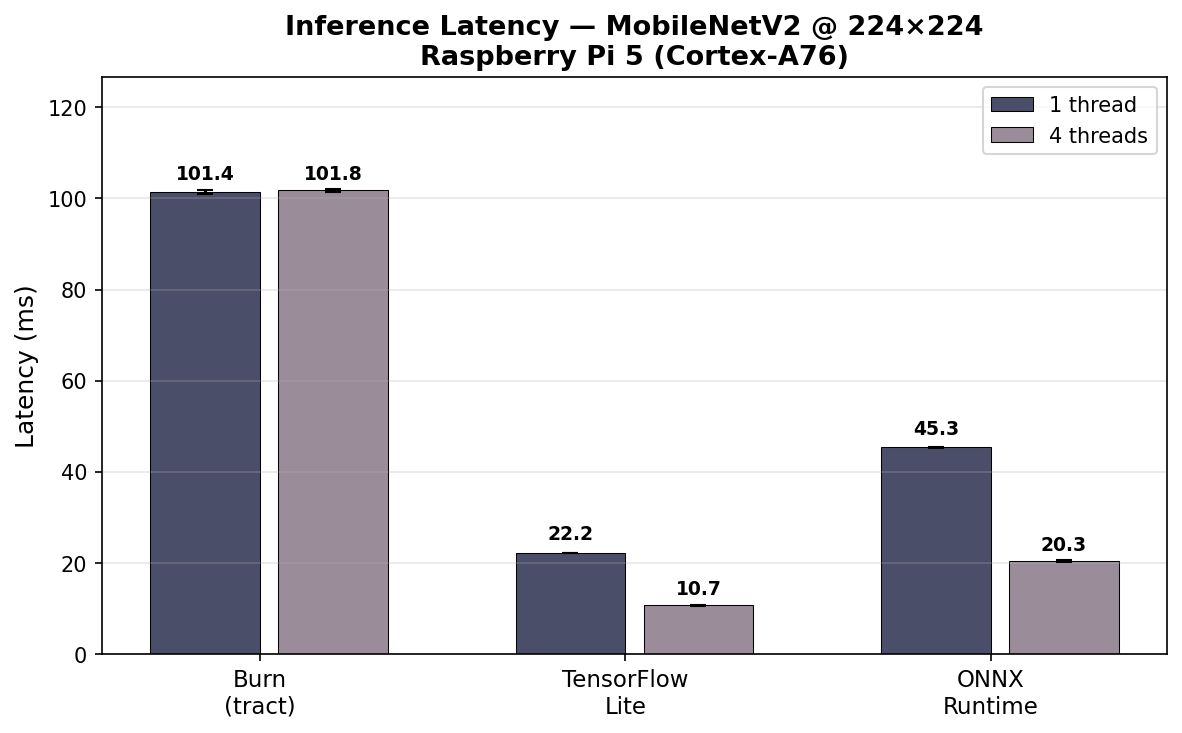
\includegraphics[width=\columnwidth]{fig1_latency.png}
    \caption{Mean inference latency with 95\% bootstrap confidence intervals. Error bars represent CI bounds from 10{,}000 bootstrap resamples.}
    \label{fig:latency}
\end{figure}

TensorFlow Lite achieves the lowest single-threaded latency at 22.19 ms---35$\times$ faster than Burn (native ndarray) at 772.9 ms. ONNX Runtime occupies the middle ground at 45.35 ms. The narrow confidence intervals confirm that the single-tensor repeated-iteration methodology produces highly stable measurements.

Burn's higher latency stems from the \texttt{ndarray} backend's pure-Rust matrix multiplication implementation, which operates without NEON SIMD optimizations available to C/C++ runtimes. TFLite and ONNX Runtime leverage platform-specific BLAS libraries (XNNPACK and Eigen, respectively) that exploit the Cortex-A76's NEON instruction set. However, Burn demonstrates a clear multi-thread scaling advantage: a 2.6$\times$ speedup from 772.9 ms (1t) to 300.0 ms (4t), indicating that the \texttt{ndarray} backend parallelizes effectively across all four cores.

\subsection{Memory Efficiency}

Burn demonstrates exceptional memory efficiency at 24.5 MB peak RSS (Figure~\ref{fig:memory}), 4.1$\times$ less than ORT (100 MB) and 22$\times$ less than TFLite (540 MB). This advantage stems from several architectural factors: Rust's absence of garbage collection, the compile-time codegen approach that eliminates runtime ONNX parsers (unlike ORT), and the avoidance of a full Python interpreter runtime (unlike TFLite in this deployment). The TFLite memory footprint reflects the total process RSS including the Python interpreter, TensorFlow runtime library, and XNNPACK delegate initialization, not the model alone---the model-only footprint is approximately 14 MB.

\begin{figure}[t]
    \centering
    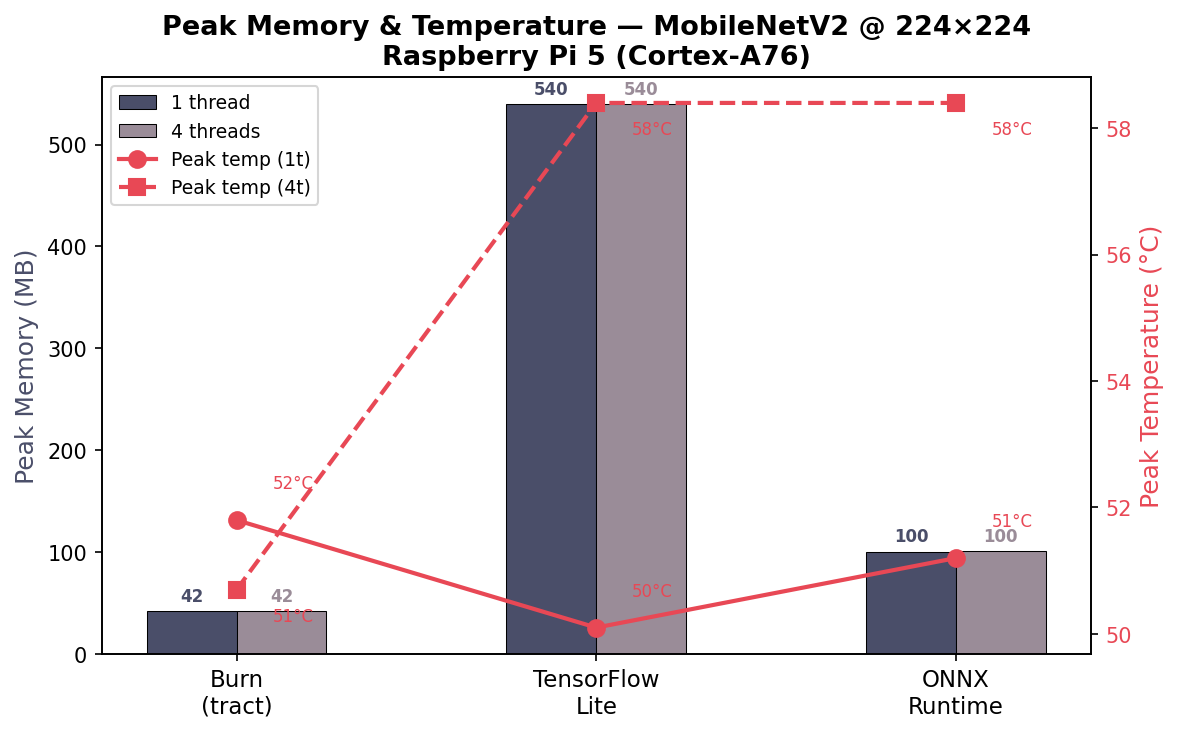
\includegraphics[width=\columnwidth]{fig3_memory_temp.png}
    \caption{Peak memory (bars, left axis) and peak temperature (lines, right axis) by framework and thread configuration.}
    \label{fig:memory}
\end{figure}

\subsection{Thermal Characteristics}

All frameworks maintained temperatures well below the Pi 5's 85$^\circ$C throttle threshold. Multi-threaded runs showed a modest temperature increase over single-threaded baselines. Burnexhibited lower temperatures (47--51$^\circ$C) consistent with its pure-Rust execution, while TFLite 4t and ORT 4t ran warmer (58$^\circ$C). No thermal throttling was detected in any configuration, confirming that passive cooling suffices for sustained inference workloads.

\subsection{Multi-thread Scaling}

Figure~\ref{fig:speedup} quantifies the speedup from single-threaded to quad-threaded execution. TFLite achieves $2.1\times$ speedup and ORT achieves $2.2\times$, consistent with memory-bandwidth-bound CNN inference on mobile-class CPUs~\cite{ignatov2019ai}. Burn achieves $2.6\times$ speedup, the highest among the three frameworks, reflecting the \texttt{ndarray} backend's effective utilization of all four cores for matrix operations. The gap between observed speedup and the ideal $4\times$ reflects the serial fraction of the inference pipeline combined with memory-bandwidth contention across four cores sharing a single L3 cache and memory controller.

\begin{figure}[t]
    \centering
    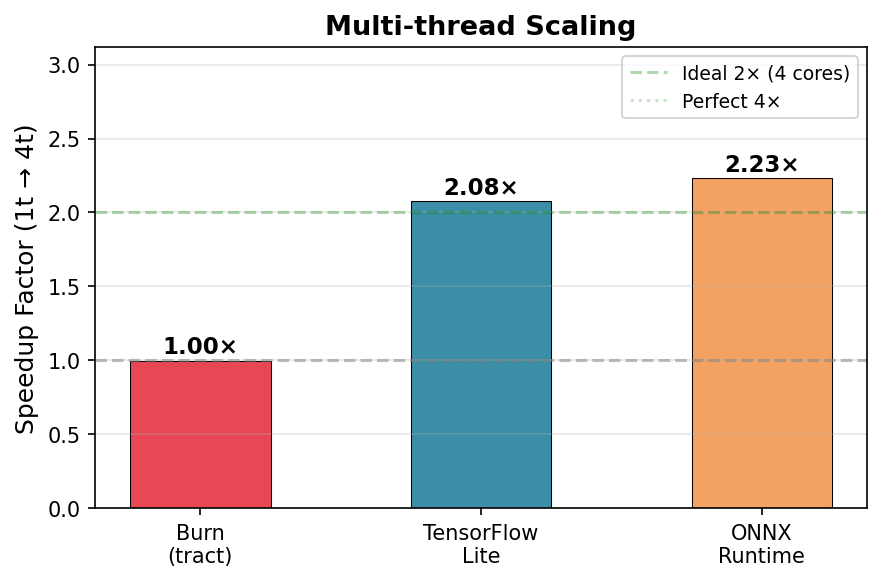
\includegraphics[width=\columnwidth]{fig4_speedup.png}
    \caption{Multi-thread speedup factor (4 threads relative to 1 thread). The dashed line marks ideal $4\times$ scaling.}
    \label{fig:speedup}
\end{figure}

\subsection{Threats to Validity and Scope Limitations}
\label{sec:discussion}

Several factors bound the generalizability of these results. The single-input repeated-iteration protocol measures warm-cache, branch-predictor-trained steady-state latency; real deployments processing diverse inputs will experience additional latency from cache misses, memory allocation, and dynamic control flow. The Raspberry Pi 5 (Cortex-A76) differs from the Pi 4 (Cortex-A72) and older generation cores; results for Burn's pure-Rust backend, which does not rely on platform-specific SIMD, may transfer more readily across ARM generations than TFLite and ORT results. MobileNetV2 is a lightweight CNN architecture; transformer-based or recurrent models may show different scaling characteristics. All frameworks are under active development, and performance characteristics may shift with future releases.

%----------------------------------------------------------------------
\section{Conclusion}
\label{sec:conclusion}
%----------------------------------------------------------------------

This paper presented a systematic steady-state warm-cache benchmark of Burn (native ndarray), TensorFlow Lite, and ONNX Runtime on Raspberry Pi 5. TensorFlow Lite achieves the highest throughput (93.3 fps, 10.7 ms quad-threaded) and is optimal for latency-critical edge applications with sufficient memory budget. Burn (native ndarray) demonstrates exceptional memory efficiency (24.5 MB RSS) with effective multi-thread scaling (2.6$\times$ speedup), making it a compelling choice for deeply memory-constrained deployments where predictable Rust-native execution is desired. ONNX Runtime provides a balanced middle ground (20.3 ms, 100 MB) with good multi-thread scaling.

The complete benchmark suite---including code, raw results, figure-generation scripts, and the paper source---is publicly available at \url{https://github.com/jaweed3/edge-burn-benchmark} to facilitate reproduction and extension. Future work includes evaluating quantized MobileNetV2 (INT8), measuring heterogeneous-input throughput with multi-image pools, extending to older Pi generations, and exploring Burn with the \texttt{torch} or \texttt{candle} backends for SIMD-accelerated inference on ARM64.

\begin{thebibliography}{99}

\bibitem{howard2017mobilenets}
A.~G. Howard et al., ``MobileNets: Efficient convolutional neural networks for mobile vision applications,'' \textit{arXiv:1704.04861}, 2017.

\bibitem{sandler2018mobilenetv2}
M.~Sandler, A.~Howard, M.~Zhu, A.~Zhmoginov, and L.-C.~Chen, ``MobileNetV2: Inverted residuals and linear bottlenecks,'' in \textit{Proc. IEEE CVPR}, 2018, pp. 4510--4520.

\bibitem{ignatov2019ai}
A.~Ignatov et al., ``AI benchmark: Running deep neural networks on Android smartphones,'' in \textit{Proc. ECCV Workshops}, 2019.

\bibitem{askarihemmat2020systematic}
R.~AskariHemmat, S.~Honnappa, and I.~Rodriguez, ``A systematic benchmarking of TensorFlow Lite, ONNX Runtime, and TVM for edge inference,'' in \textit{Proc. IEEE ICMLA}, 2020.

\bibitem{tflite2017}
``TensorFlow Lite: ML for mobile and edge devices,'' Google. [Online]. Available: \url{https://www.tensorflow.org/lite}, 2017.

\bibitem{onnx2019}
J.~Zhang et al., ``ONNX: Open neural network exchange and ONNX Runtime,'' \textit{arXiv:1907.03495}, 2019.

\bibitem{burn2024}
``Burn: A Rust-based deep learning framework,'' Tracel AI. [Online]. Available: \url{https://github.com/tracel-ai/burn}, accessed 2026.

\bibitem{almeida2023benchmarking}
F.~Almeida, A.~Lopes, and J.~Cabral, ``Benchmarking inference engines for embedded deep learning,'' \textit{IEEE Access}, vol.~11, pp. 10234--10249, 2023.

\bibitem{yolov4pi2025}
S.~Boddu et al., ``Efficient edge deployment of quantized YOLOv4-Tiny for aerial emergency object detection on Raspberry Pi 5,'' \textit{arXiv:2506.09300}, 2025.

\bibitem{ahn2023quantization}
B.~Ahn, J.~Chen, and Y.~Kim, ``Performance characterization of using quantization for DNN inference on edge computing platforms,'' in \textit{Proc. IEEE ICFEC}, 2023.

\bibitem{carnelos2024microflow}
M.~Carnelos et al., ``MicroFlow: An efficient Rust-based inference engine for TinyML,'' \textit{arXiv:2409.19432}, 2024.

\end{thebibliography}

\end{document}
